%% ----------------------------------------------------------------
%% OverallApproach.tex
%% ---------------------------------------------------------------- 
\chapter{Overall Approach} 
\label{Chapter:Overall Approach}
\section{Client Requirements}
With the end aim of integrating this project into the new version of Synote there were some specific requirements that our client had with regards to implementation.

The overlaid video player must be written in AngularJS and HTML5 to make it easily compatible with the new version of Synote. From our analysis of available HTML5 video players it was agreed that \gls{Videogular} should be used.

Video polls must also be included.

\subsection{Synote}
\label{Section:Synote}
Synote\footnote{\url{http://www.synote.org/synote/} (Accessed: 14 Jan 15)} is a web multimedia annotation system designed with accessibility in mind. 

The application aims to make multimedia content accessible by synchronising the multimedia in many different formats (see \autoref{Figure:Synote}). The formats used are textual, video/audio, bookmarks and images. 

\begin{figure}[h!]
	\centering 
		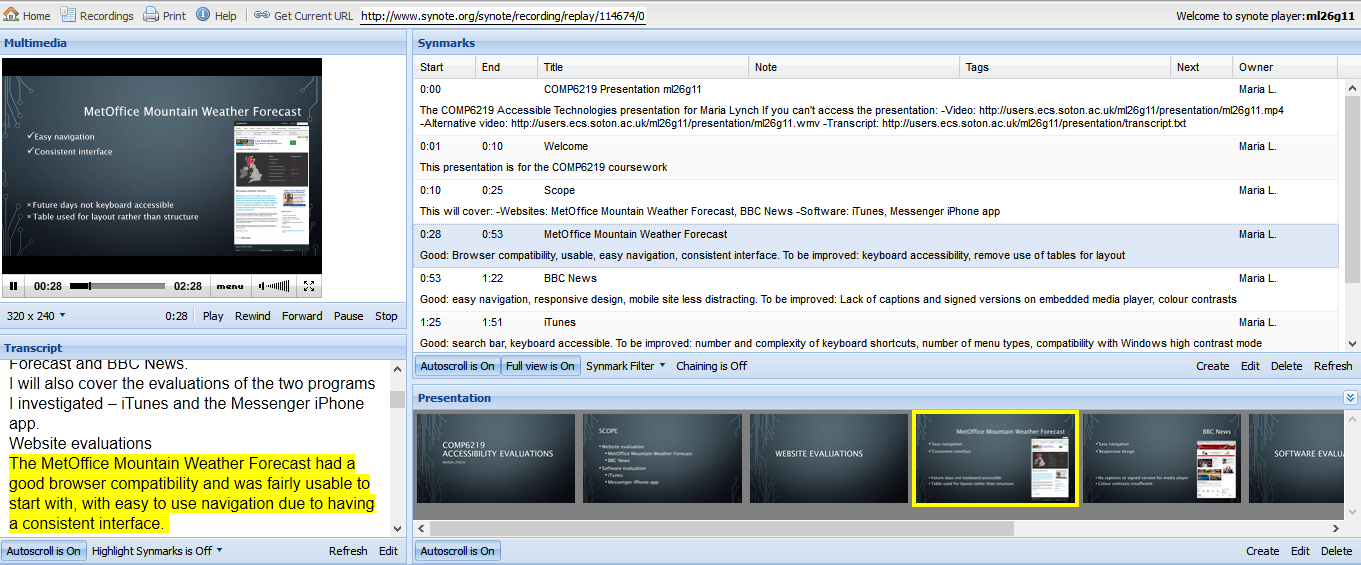
\includegraphics[scale=0.4]{../figures/synote_sync.png} 		
	\caption{\label{Figure:Synote} Screenshot of a Synote replay correctly synchronised (\url{http://www.synote.org/synote/recording/replay/114674/0} (Accessed: 15 Jan 15))}
\end{figure}

The textual element is a transcript of the video/audio. This aims to make the presentations more accessible for people with hearing impairments and cognitive difficulties. It also makes the presentation more easily searchable.

The bookmarks (known as Synmarks) can be used for many reasons. For example they could be used to provide summaries of the slides, make notes on the presentation or provide a direct copy of the text from the slides.

The images can be PowerPoint slides that are used in the presentation so that there can be other video to explain the slides at the same time.

Using the print function a screen reader friendly version of the presentation can be produced\footnote{\url{http://www.synote.org/synote/recording/handlePrint?id=114674&_part=&part=on&from=&to=&_synmarked=&_synmarked-user-1771=&_transcript=&transcript=on&_presentation=&presentation=on&slideHeight=&_synmarks=&synmarks=on&_synmarks-user-1771=&synmarks-user-1771=on&_synmarkId=&synmarkId=on&_synmarkTiming=&synmarkTiming=on&_synmarkTitle=&synmarkTitle=on&_synmarkNote=&synmarkNote=on&_synmarkTags=&synmarkTags=on&_synmarkOwner=&synmarkOwner=on&_synmarkNext=&synmarkNext=on}(Accessed: 15 Jan 15)}. This provides the transcripts, bookmarks and images in sequential order so that a screen reader can read all the text. This will be particularly useful to visually impaired users.
\subsection{AngularJS}
\label{Section:AngularJS}
\gls{AngularJS}\footnote{\url{https://angularjs.org/}} is a JavaScript Framework that extends HTML attributes. It is an open source library made by Google.

The underlying architectural pattern used by \gls{AngularJS} is client side \gls{MVC}. This is where the data (model), appearance (view) and actions that can be applied (controller) are separated out to make encapsulation and code reuse easier. 

The framework allows custom HTML tags and attributes to be created using directives. Directives allow the user to specify the behaviour of specific elements they have created.

One of \gls{AngularJS}'s most prominent features is its use of two-way binding. This synchronises the views with the data held in the model. This is especially useful when dealing with dynamic content as when extra content is added it is automatically shown in the view.

\subsection{Videogular}
\label{Section:Videogular}
\gls{Videogular}\footnote{\url{https://github.com/2fdevs/videogular}}\footnote{\url{https://github.com/2fdevs/bower-videogular-controls}} provides a HTML5 video player for \gls{AngularJS}. The nature of the library makes it very easy to write plugins for this to get the extra functionality required.

\section{Stakeholder Analysis}
For an approach for the project to be decided on the stakeholders needed to be identified and analysed. Their requests have been prioritised by categorising each stakeholder (see \autoref{fig:Stakeholder matrix}).
\begin{figure}[h!]
\centering
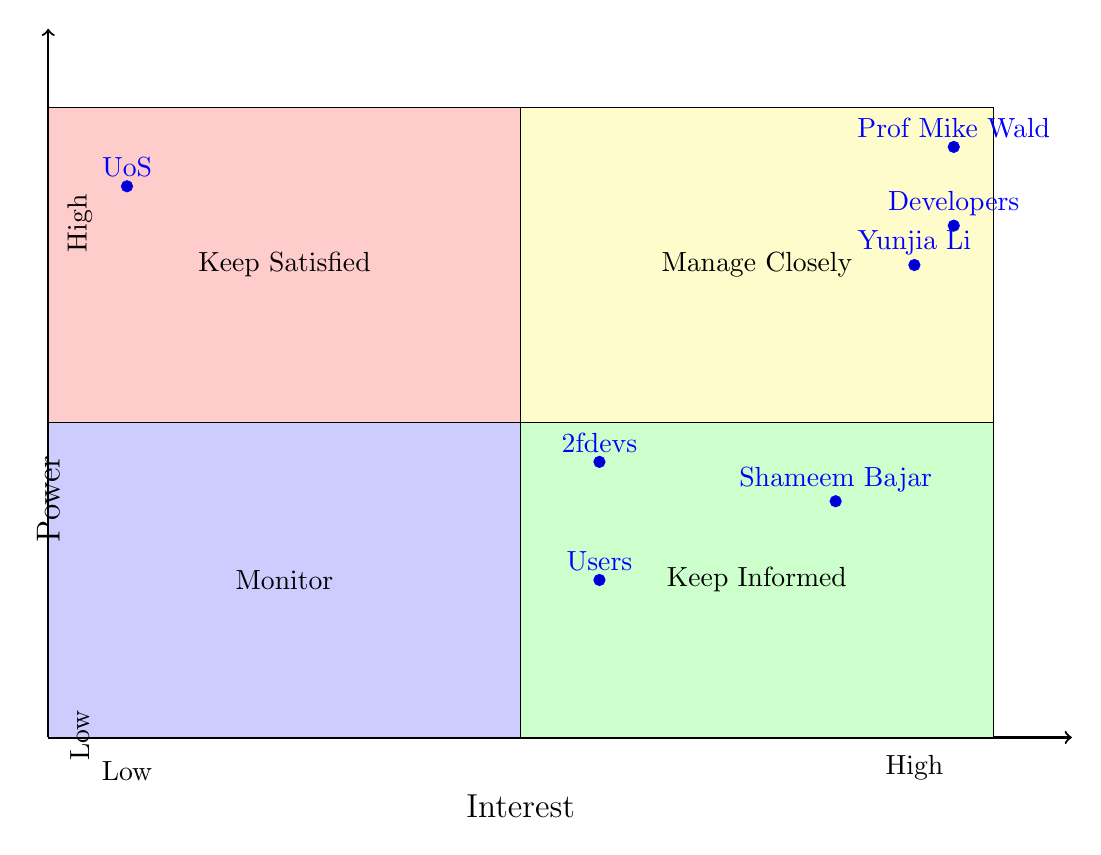
\begin{tikzpicture}[font=\rmfamily]
\draw [thick,->]  (0,0) -- coordinate (x axis mid) (13,0);
\draw [thick,->]  (0,0) -- coordinate (y axis mid) (0,9);
\filldraw[fill=blue!20!white, draw=black] (0,0) rectangle (6,4) node[pos=.5] {Monitor};
\filldraw[fill=green!20!white, draw=black] (6,0) rectangle (12,4) node[pos=.5] {Keep Informed};
\filldraw[fill=red!20!white, draw=black] (0,4) rectangle (6,8) node[pos=.5] {Keep Satisfied};
\filldraw[fill=yellow!20!white, draw=black] (6,4) rectangle (12,8) node[pos=.5] {Manage Closely};
%labels      
\node[xshift=-0.5cm, below=0.6cm] (xlabel) at (x axis mid) {{\large Interest}};
\node[rotate=90, left=0.8cm] (ylabel) at (y axis mid) {{\large Power}};
\begin{axis}[nodes near coords, xmin=0, xmax=13, ymin=0, ymax=9, width=13cm, height=9cm, axis x line=none, axis y line=none, scale only axis, enlargelimits=false]
\addplot+[only marks, point meta=explicit symbolic] coordinates { 
(11.5,7.5) [Prof Mike Wald] 
(7,3.5) [2fdevs] 
(10,3) [Shameem Bajar] 
(11,6) [Yunjia Li] 
(11.5,6.5) [Developers] 
(7, 2) [Users]
(1,7) [UoS]
 };
\end{axis}
\node[xshift=-5cm, above=0.2cm] at (xlabel) {Low};
\node[xshift=5cm, above=0.2cm] at (xlabel) {High};
\node[xshift=0.4cm,yshift=-3cm, rotate=90] at (ylabel) {Low};
\node[xshift=0.4cm,yshift=3.5cm, rotate=90] at (ylabel) {High};
\end{tikzpicture}
\caption{Stakeholder matrix for the project\label{fig:Stakeholder matrix}}
\end{figure}

Our supervisor and client, Professor Mike Wald, had the most interest and power in the project. As the project proposer it would be his ideas that would form the basis of the project.

Yunjia Li is the lead developer for the new version of Synote. As the aim of the project was to provide code that could be used within this he had a lot of interest in the project. His requirements would need to be taken into account to ensure interoperability between the two systems, which gave him power in the project.

Due to the nature of the project the developers on the project would be major stakeholders. All work would need to be evenly distributed to allow all members of the group to attain the same marks.

The University of Southampton sets the mark scheme and guidelines for the project. These would need to be satisfied to make the project successful.

2fdevs are the development team who created the \gls{Videogular} player. The project would be creating plugins for this player so would rely on certain attributes of \gls{Videogular} such as accessibility. 

Shameem Bajar is a 3rd year student who has an Individual Project based around this project. Her interest levels would be high as her work depends on the output of this project. 

The users would be interested in the outcome of the project as the decisions made will affect how easy the system is to use and whether all of the desired functionality is available.

Requirements from all stakeholders will be considered but any conflicts will be dealt with by prioritising the needs of the most influential party (closer to the top right of \autoref{fig:Stakeholder matrix}).

\section{Requirements Analysis}
\label{Section:Requirements Analysis}
Looking at the needs of all the stakeholders a set of requirements for the project were agreed.
\subsection{Functional Requirements}
\begin{requirement}[label=\textbf{F\arabic*}]
\item \textbf{Question types}  \hfill \\ The overlaid video player must be able to display single choice, multiple choice, range selector, rating and text based answer types\label{Req:Question types}
\item \textbf{Jumping to content} \hfill \\ There should be a feature to jump to specific content if a question is answered incorrectly \label{Req:Jumping to content}
\item \textbf{Analytics events} \hfill \\ Video and question events should be emitted from the overlaid video player in order than analytics data can be calculated \label{Req:Analytics events}
\item \textbf{Cuepoints} \hfill \\ The locations of the questions should be marked visually on the scrub bar of the video \label{Req:Cuepoints}
\item \textbf{Poll responses} \hfill \\ The responses to polls must be able to be sent to and recorded on a server to allow viewing of the results \label{Req:Poll responses}
\end{requirement}

\subsection{Non-Functional Requirements}
\begin{requirement}[label=\textbf{N\arabic*}]
\item \textbf{Video player used} \hfill \\ Videogular should be used as the video player with components written in AngularJS and HTML5 \label{Req:Video player used}
\item \textbf{Standalone} \hfill \\ The plugins created should be standalone code but still be easy to integrate into the new version of Synote \label{Req:Standalone}
\item \textbf{Browser compatibility} \hfill \\ The overlaid video player must work on Internet Explorer, Firefox and Chrome \label{Req:Browser compatibility}
\item \textbf{Operating System Compatibility} \hfill \\ The overlaid video player must work on Windows, OSX and Android \label{Req:OS compatibility}
\item \textbf{Extensibility} \hfill \\ The overlaid video player must be extensible so that further features can be added \label{Req:Extensibility} 
\item \textbf{Keyboard Accessibility} \hfill \\ The overlaid video player and authoring tool must be completely accessible to a keyboard-only user \label{Req:Keyboard accessibility}
\item \textbf{Use of colour} \hfill \\ Any colours used should be customisable \label{Req:Use of colour}
\item \textbf{User interface} \hfill \\ A Graphical User Interface (GUI) must be provided for the Authoring Tool so that non-technical users can create quizzes \label{Req:User interface}
\item \textbf{Documentation} \hfill \\ The plugins built should have usage examples documented to allow less technical users to implement their own system \label{Req:Documentation}
\item \textbf{Server architecture} \hfill \\ Any server behaviour should be accessed by \gls{REST} calls with no requirement that all servers should be on the same host \label{Req:Server architecture}
\end{requirement}

\section{Modular Webserver Approach}
\label{Section:Modular Approach}
It is important for our project to be easily integrated into other projects, specifically we are looking to have it integrated into the latest version of Synote (see \autoref{Section:Synote}). To accomplish this we have designed the back end systems to ensure they can be run without depending on any other modules. All of the functionality will be able to be accessed by \gls{REST} calls.

By abstracting all calls to using \gls{REST} this means that other services will be able to interact with out back end services in a language independent way. To facilitate this we have had to ensure that all \gls{REST} responses are returned with a Cross-Origin header. This allows servers who are not on the same machine to be able to communicate with the \gls{REST} service.

These features will allow an external application to be able to run the webserver separately and communicate with our server side code. This ensures that the only dependency added by those that use our code will be that they need to be able to make \gls{REST} calls.

\section{System Architecture}
As the expected behaviour of our plugins would depend on the application they were used in a set of examples would be required to test our plugins. The following set of deliverables was agreed in order to meet the requirements:
\begin{itemize}
\item Videogular Questions: a plugin for adding polls and questions to videos
\begin{itemize}
\item Source code, under the MIT licence
\item An example proof-of-concept website
\end{itemize}
\item Videogular Cuepoints: a plugin which displays informational marks on the scrub bar of a video
\begin{itemize}
\item Source code, under the MIT licence
\item Demonstration of usage in Videogular Questions example site
\end{itemize}
\item Videogular Analytics: a plugin for reporting of events within the Videogular player
\begin{itemize}
\item Source code, under the MIT licence
\item An API specification for Videogular Analytics
\item An example site showing basic usage of the analytics data collected from the plugin
\end{itemize}
\item Videogular Heatmap: a plugin which displays heat map information on the scrub bar of a video
\begin{itemize}
\item Source code, under the MIT licence
\item Demonstration of usage in Videogular Analytics example site
\end{itemize}
\item Authoring tool: a Web application to produce the JavaScript file to be used with Videogular Questions
\begin{itemize}
\item Source code, under the MIT licence
\end{itemize}
\end{itemize}

These elements would have a range of interactions (see \autoref{fig:System architecture diagram}).

\todo{The arrows all need some form of labels, or reasons why some don't and some do}
\begin{figure}[h!]
\centering
\begin{tikzpicture}[
  font=\sffamily,
  every matrix/.style={ampersand replacement=\&,column sep=2cm,row sep=2cm},
  source/.style={draw,thick,rounded corners,fill=yellow!20,inner sep=.3cm},
  vg-plugin/.style={draw,thick,rounded corners,fill=yellow!20,inner sep=.3cm},
  videogular/.style={draw,thick,circle,fill=blue!20},
  process/.style={draw,thick,circle,fill=blue!20},
  sink/.style={source,fill=green!20},
  datastore/.style={draw,very thick,shape=datastore,inner sep=.3cm},
  server/.style={source,fill=green!20},
  dots/.style={gray,scale=2},
  to/.style={->,>=stealth',shorten >=1pt,semithick,font=\sffamily\footnotesize},
  between/.style={<->,>=stealth',shorten >=1pt,semithick,font=\sffamily\footnotesize},
  every node/.style={align=center}]

  % Position the nodes using a matrix layout
  \matrix{
    \node[vg-plugin] (cuepoints) {cuepoints};
      \&
      \& \node[vg-plugin] (questions) {questions};
      \& \node[server] (poll-server) {poll server}; \\

    \& \node[videogular] (videogular) {videogular}; \\

    \node[vg-plugin] (heatmap) {heatmap};
      \&
      \& \node[vg-plugin] (analytics) {analytics};
      \& \node[server] (analytics-server) {analytics server}; \\
  };

  \draw[between] (questions) --
      node[midway,above] {user responses}
      node[midway,below] {results} (poll-server);
  \draw[to] (questions) --
      node[midway,right] {user interactions}
      (analytics);
  \draw[to] (questions) --
      node[midway,above] {question times}
      (cuepoints);
  \draw[between] (analytics) --
      node[midway,above] {data}
      node[midway,below] {acks} (analytics-server);
  \draw[to] (analytics-server) to[bend left=15] node[midway,above] {events}
      node[midway,below] {level 1} (heatmap);
  \draw[between] (videogular) -- (cuepoints);
  \draw[between] (videogular) -- (analytics);
  \draw[between] (videogular) -- (questions);
  \draw[between] (videogular) -- (heatmap);
\end{tikzpicture}

\caption{System architecture diagram for the project \label{fig:System architecture diagram}}
\end{figure}

